\documentclass[letter,11pt]{article}

\usepackage[spanish,es-nodecimaldot]{babel}
\usepackage[utf8]{inputenc}

\usepackage{lmodern}
\usepackage[T1]{fontenc}
\usepackage{textcomp}

\usepackage{framed}
\usepackage[svgnames]{xcolor}
\colorlet{shadecolor}{Gainsboro!50}

\usepackage{enumitem}
\usepackage{graphicx}
\usepackage{pstricks}

\usepackage{anysize}
\marginsize{3cm}{2cm}{2cm}{3cm}

\usepackage{siunitx}
\usepackage{amsmath}
\usepackage{array}
\usepackage{alltt}

\usepackage{fancyhdr}
\usepackage{lastpage}
\pagestyle{fancy}
\fancyhf{}
\fancyhead[LE,RO]{Física Básica II}
\fancyfoot[CO,CE]{\thepage\ de \pageref{LastPage}}

\special{papersize=215.9mm,279.4mm}

\usepackage[
    pdfauthor={Carlos Eduardo Caballero Burgoa},%
    pdftitle={Física Básica II},%
    pdfsubject={Tarea 3},%
    colorlinks,%
    citecolor=black,%
    filecolor=black,%
    linkcolor=black,%
    urlcolor=black,
    breaklinks]{hyperref}
\usepackage{breakurl}

\newcommand{\blankpage}{
\newpage
\thispagestyle{empty}
\mbox{}
\newpage
}

\renewcommand{\arraystretch}{1.2}

\begin{document}

\begin{center}
    {\Large \bf{\underline{Tarea \#3}}}
\end{center}

Supongamos un sistema discreto de dos partículas, donde $m_1 \ll m_2$ y están
separados por una distancia $d$.

\begin{figure}[!h]
\centering
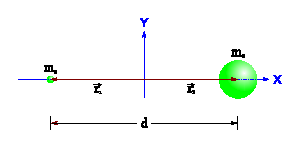
\includegraphics[scale=2.5]{resources/f1.eps}
\end{figure}

Calcular:

\begin{enumerate}[label=(\alph*)]
    \item la relación exacta del centro de masa de ambas partículas.
    \item una relación aproximada del centro de masa si $m_1 \ll m_2$.
    \item el centro de masa exacta (a) y aproximada (b) del sistema
        Sol-Tierra. \\
        Si: $m_s = \num{1.989e30} [kg]$, $r_s = 696340 [km]$,
        $d = \num{149.6e6} [km]$, $m_t = \num{5.9736e24} [kg]$ y
        $r_t = 6371 [km]$. ¿Dónde esta ubicado el centro de masa de este
        sistema?
\end{enumerate}

\textbf{\underline{Solución}:} \\

(a)

\begin{equation*}
    \vec{r}_{cm} = \frac{1}{M} \sum_{i=1}^{n} m_i \vec{r}_i
\end{equation*}
\begin{equation*}
    \vec{r}_{cm} = \frac{m_1 \vec{r}_1 + m_2 \vec{r}_2}{m_1 + m_2}
\end{equation*}

Descomponiendo en sus componentes $x$ y $y$:
\begin{equation*}
    x_{cm} = \frac{m_1 x_1 + m_2 x_2}{m_1 + m_2}
\end{equation*}
\begin{equation*}
    y_{cm} = \frac{m_1 y_1 + m_2 y_2}{m_1 + m_2} = 0
\end{equation*}

Si movemos el sistema de referencia hacia el centro de la masa $m_1$,
hallamos la siguiente:
\begin{equation}
    x_{cm} = \frac{m_2 d}{m_1 + m_2}
\label{exacta}
\end{equation}

\vspace{0.5cm}
(b)

Si $m_1 \ll m_2$, podemos asumir:
\begin{equation*}
    m_1 + m_2 \approx m_2
\end{equation*}

Resultando:
\begin{equation}
    x_{cm} \approx d
\label{aproximada}
\end{equation}

Es decir, que el centro de masa total del sistema tiende al centro de masa $m_2$
a mayor diferencia exista entre ambas.

\vspace{0.5cm}
(c)

\begin{figure}[!h]
\centering
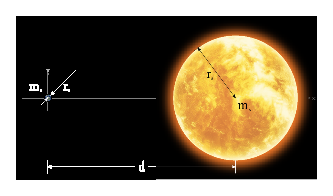
\includegraphics[scale=2.75]{resources/f2.eps}
\end{figure}

Calculando el centro con la ecuación (\ref{exacta}), obtenemos:
\begin{equation*}
    x_{cm} = \frac{m_s d}{m_t + m_s} = \frac{(\num{1.989e30}) (\num{149.6e6})}{\num{5.9736e24}+\num{1.989e30}} = \num{149.6e6} [km]
\end{equation*}

Mientras que con la ecuación (\ref{aproximada}), el resultado es:
\begin{equation*}
    x_{cm} \approx d = \num{149.6e6} [km]
\end{equation*}

Calculando la diferencia entre la distancia y el centro de masa, obtenemos:
\begin{equation}
    d - x_{cm} = 449.30 [km]
\end{equation}

Por tanto el centro de masa del sistema, se encuentra a $449.30 [km]$ del centro
del sol, que considerando las distancias utilizadas es una cantidad despreciable.

\end{document}

